\documentclass{standalone}
\usepackage{tikz}
\usepackage{ctex,siunitx}
\setCJKmainfont{Noto Serif CJK SC}
\usepackage{tkz-euclide}
\usepackage{amsmath}
\usetikzlibrary{patterns, calc,3d}
\usetikzlibrary {decorations.pathmorphing,decorations.pathreplacing,decorations.shapes}
\tikzset{label style/.append style={font=\small}}
\begin{document}
\small
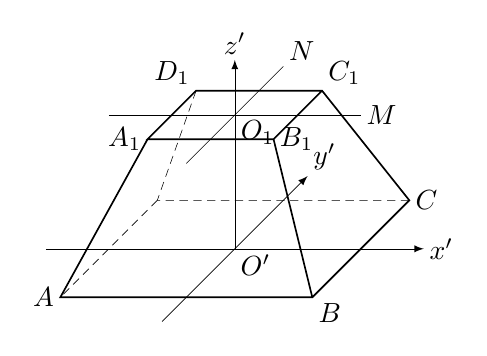
\begin{tikzpicture}[>=latex,scale=0.8,inner sep=2pt]
  \draw[semithick](-1,2.125,1)node[left]{$A_1$}--(-2,0,2)node[left]{$A$}--(2,0,2)node[below right]{$B$}--(2,0,-2)node[right]{$C$}--(1,2.125,-1)node[above right]{$C_1$}--(-1,2.125,-1)node[above left]{$D_1$}--(-1,2.125,1)--(1,2.125,1)node[right]{$B_1$}--(1,2.125,-1)(2,0,2)--(1,2.125,1);
  \node at (0,2.125,0)[below right]{$O_1$};
  \draw[very thin,](-2,2.125,0)--(2,2.125,0)node[right]{$M$};
  \draw[very thin,](0,2.125,2)--(0,2.125,-2)node[above right]{$N$};
  \draw[very thin,->](-3,0,0)--(3,0,0)node[right]{$x'$};
  \draw[very thin,->](0,0,3)--(0,0,-3)node[above right]{$y'$};
  \draw[very thin,->](0,0,0)node[below right]{$O'$}--(0,3,0)node[above]{$z'$};
  \draw[very thin,densely dashed] (-1,2.125,-1)--(-2,0,-2)--(2,0,-2)(-2,0,-2)--(-2,0,2);
\end{tikzpicture}
\end{document}